\documentclass[11pt,a4paper]{article}

% ---------- Packages ----------
\usepackage[T1]{fontenc}
\usepackage[utf8]{inputenc}
\usepackage[margin=2.5cm]{geometry}
\usepackage{graphicx}
\usepackage{xcolor}
\usepackage{tikz}
\usetikzlibrary{arrows.meta,positioning,shapes.geometric,fit,backgrounds,calc}
\usepackage{pgfplots}
\pgfplotsset{compat=1.18}
\usepackage{booktabs}
\usepackage{array}
\usepackage{longtable}
\usepackage{listings}
\usepackage{caption}
\usepackage{enumitem}
\usepackage{titlesec}
\usepackage{fancyhdr}
\usepackage{amssymb}
\usepackage{float}
\usepackage[hidelinks,colorlinks=true,linkcolor=NavyBlue,citecolor=NavyBlue,urlcolor=NavyBlue]{hyperref}

% ---------- Colors ----------
\definecolor{NavyBlue}{RGB}{0,51,102}
\definecolor{AgentBlue}{RGB}{209,229,255}
\definecolor{OrchOrange}{RGB}{255,224,178}
\definecolor{StoreGray}{RGB}{230,230,230}
\definecolor{RealGreen}{RGB}{205,235,205}
\definecolor{BugRed}{RGB}{255,214,214}
\definecolor{CodeBg}{RGB}{245,245,245}
\definecolor{CodeKeyword}{RGB}{0,90,180}
\definecolor{CodeComment}{RGB}{110,110,110}
\definecolor{CodeString}{RGB}{160,40,40}

% ---------- Section styling ----------
\titleformat{\section}{\Large\bfseries\color{NavyBlue}}{\thesection}{0.5em}{}
\titleformat{\subsection}{\large\bfseries\color{NavyBlue!80!black}}{\thesubsection}{0.5em}{}

% ---------- Headers/footers ----------
\pagestyle{fancy}
\fancyhf{}
\fancyhead[L]{\small OpenEdu Orchestrator -- Implementation Report (Revision 2)}
\fancyhead[R]{\small \thepage}
\renewcommand{\headrulewidth}{0.4pt}

% ---------- Code listing styles ----------
\lstdefinestyle{pystyle}{
    backgroundcolor=\color{CodeBg},
    basicstyle=\ttfamily\footnotesize,
    keywordstyle=\color{CodeKeyword}\bfseries,
    commentstyle=\color{CodeComment}\itshape,
    stringstyle=\color{CodeString},
    numbers=left,
    numberstyle=\tiny\color{gray},
    numbersep=8pt,
    frame=single,
    rulecolor=\color{gray!50},
    breaklines=true,
    showstringspaces=false,
    tabsize=4,
    language=Python,
    xleftmargin=1.2em,
}

\lstdefinestyle{termstyle}{
    backgroundcolor=\color{black!92},
    basicstyle=\ttfamily\footnotesize\color{white},
    frame=single,
    rulecolor=\color{gray!50},
    breaklines=true,
    showstringspaces=false,
    xleftmargin=1.2em,
}

\lstset{style=pystyle}

\newcommand{\ttu}[1]{\texttt{\detokenize{#1}}}

% ---------- Title page info ----------
\title{
    \vspace{-2cm}
    {\Huge \bfseries \color{NavyBlue} OpenEdu Orchestrator}\\[0.4cm]
    {\Large An Agentic Multi-Agent Data Synchronization System}\\[0.2cm]
    {\large PIEAS $\rightarrow$ OpenEduCat (Odoo) ERP}\\[0.3cm]
    {\normalsize \itshape Implementation Report, Revision 2 -- Real Infrastructure,
     Multi-Source Generalization, and Production Hardening}
}
\author{Muhammad Shayan Asif}
\date{\today}

% ---------- TikZ reusable styles ----------
\tikzset{
    comp/.style={draw, thick, rounded corners, fill=StoreGray, minimum width=3.3cm, minimum height=1.05cm, align=center, font=\small},
    agentbox/.style={draw, thick, rounded corners, fill=AgentBlue, minimum width=3.3cm, minimum height=1.05cm, align=center, font=\small},
    orchbox/.style={draw, thick, rounded corners, fill=OrchOrange, minimum width=3.6cm, minimum height=1.2cm, align=center, font=\small},
    realbox/.style={draw, thick, rounded corners, fill=RealGreen, minimum width=3.3cm, minimum height=1.05cm, align=center, font=\small},
    solidarr/.style={-{Latex[length=2.5mm]}, thick},
    dashedarr/.style={-{Latex[length=2.5mm]}, thick, dashed, gray!60!black},
    term/.style={draw, thick, circle, fill=gray!15, minimum size=0.95cm, font=\small},
    stage/.style={draw, thick, rounded corners, fill=AgentBlue, minimum width=4.0cm, minimum height=0.9cm, align=center, font=\small},
}

\begin{document}

\begin{titlepage}
\maketitle
\thispagestyle{empty}
\vspace{1cm}
\begin{center}
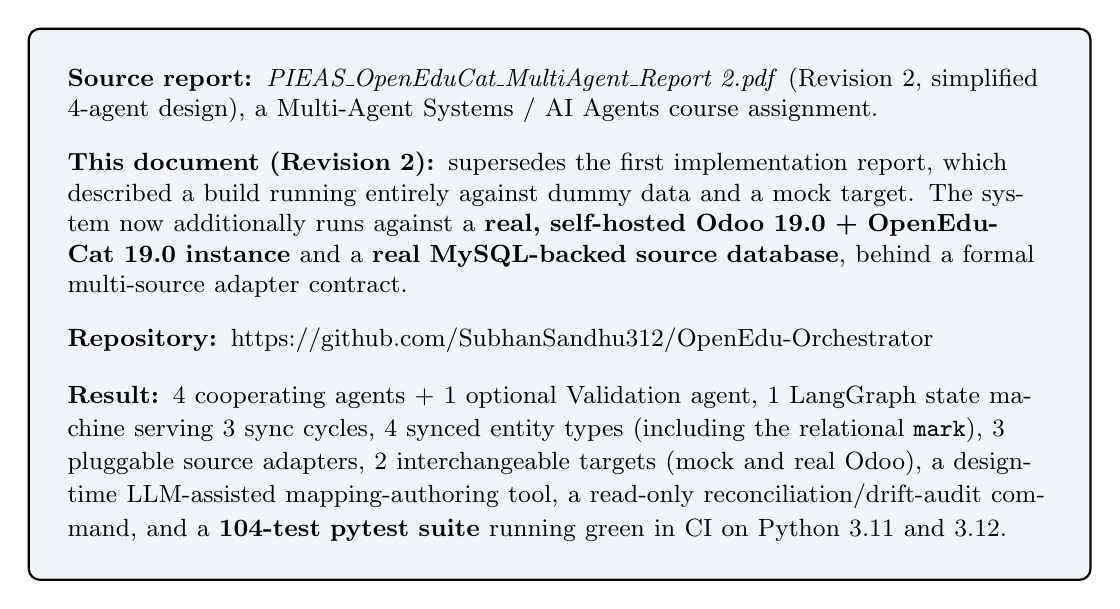
\begin{tikzpicture}
\node[draw, thick, rounded corners, fill=NavyBlue!5, align=left, text width=12.5cm, inner sep=14pt] (box) {
    \small
    \textbf{Source report:} \textit{PIEAS\_OpenEduCat\_MultiAgent\_Report 2.pdf} (Revision~2, simplified 4-agent design), a Multi-Agent Systems / AI Agents course assignment.\\[0.3cm]
    \textbf{This document (Revision~2):} supersedes the first implementation report, which described a build running entirely against dummy data and a mock target. The system now additionally runs against a \textbf{real, self-hosted Odoo 19.0 + OpenEduCat 19.0 instance} and a \textbf{real MySQL-backed source database}, behind a formal multi-source adapter contract.\\[0.3cm]
    \textbf{Repository:} \url{https://github.com/SubhanSandhu312/OpenEdu-Orchestrator}\\[0.3cm]
    \textbf{Result:} 4 cooperating agents + 1 optional Validation agent, 1 LangGraph state machine serving 3 sync cycles, 4 synced entity types (including the relational \texttt{mark}), 3 pluggable source adapters, 2 interchangeable targets (mock and real Odoo), a design-time LLM-assisted mapping-authoring tool, a read-only reconciliation/drift-audit command, and a \textbf{104-test pytest suite} running green in CI on Python 3.11 and 3.12.
};
\end{tikzpicture}
\end{center}
\vfill
\end{titlepage}

\tableofcontents
\newpage

% =========================================================================
\section{Executive Summary}
% =========================================================================

This project turns a course-assignment design document into working software. The source
report specifies an \textbf{agentic, multi-agent system} for moving data one time from the
PIEAS website into OpenEduCat (an Odoo-based Student Information System), and then keeping the
two in sync forever after -- despite PIEAS exposing no API and no webhooks of any kind.

Revision~1 of this report described a complete implementation of that design running against
deterministic dummy data and a mock OpenEduCat client. That build was correct, but every claim
about how it would behave against real systems was, necessarily, a prediction.

\textbf{Revision~2 replaces those predictions with evidence.} The same four agents now run
unchanged against a real self-hosted Odoo~19.0 + OpenEduCat~19.0 instance and a real
MySQL~source database. That exercise found five genuine defects that no amount of testing
against the mock could have surfaced (Section~\ref{sec:realbugs}) -- which is the single
strongest argument in this document for why the real-infrastructure work was worth doing.

The system as it now stands:

\begin{itemize}[leftmargin=1.4em]
    \item implements all four agents the report specifies (\textbf{Extractor}, \textbf{Transformer},
          \textbf{Loader}, \textbf{Orchestrator}) plus the optional fifth \textbf{Validation Agent},
          with the exact non-overlapping responsibilities the report defines;
    \item wires them together as a single \textbf{LangGraph} \texttt{StateGraph} serving all
          three operating cycles: bulk migration, the timestamp-watermark change cycle, and the
          full-ID-list deletion cycle;
    \item runs against \textbf{three interchangeable source adapters} behind a formal, runtime-checkable
          \texttt{SourceAdapter} Protocol -- dummy SQLite PIEAS, real MySQL PIEAS, and a second,
          genuinely distinct university source system (Section~\ref{sec:multisource});
    \item writes to \textbf{two interchangeable targets} -- the SQLite mock, and a real Odoo
          instance over XML-RPC, using Odoo's own \ttu{ir.model.data} mechanism for external-ID
          tracking (Section~\ref{sec:realtarget});
    \item ships a \textbf{design-time, LLM-assisted mapping-authoring tool} that proposes
          source$\rightarrow$target field mappings from live schema introspection, for human review --
          deliberately \emph{not} a runtime component (Section~\ref{sec:mapping});
    \item ships a read-only \textbf{reconciliation / drift-audit command} for migration cutover,
          which exits non-zero on drift so it can gate a deployment (Section~\ref{sec:reconcile});
    \item is \textbf{production-hardened}: retry/backoff on transient RPC failures, structured JSON
          logging, environment-variable credential loading, and continuous integration
          (Section~\ref{sec:hardening}); and
    \item syncs \textbf{four entity types} -- \texttt{student}, \texttt{faculty},
          \texttt{course}, and \texttt{mark}, the last being the source report's own worked
          example of an ongoing change and the first \emph{relational} entity, which required
          cross-entity dependency handling (Section~\ref{sec:refdata}); and
    \item is verified by a \textbf{104-test pytest suite} (up from 57) that remains fully
          self-contained -- no live Odoo or MySQL needed -- so it runs unmodified in CI.
\end{itemize}

% =========================================================================
\section{What Changed Since Revision 1}
% =========================================================================

For a reader familiar with the first report, this table is the fastest orientation. Everything
in the ``Revision~1'' column was true and working; the right column is what it became.

\begin{table}[H]
\centering
\small
\begin{tabular}{@{}p{3.5cm}p{5.0cm}p{6.0cm}@{}}
\toprule
\textbf{Dimension} & \textbf{Revision 1} & \textbf{Revision 2} \\
\midrule
Source system & One dummy SQLite database, hardcoded &
Three adapters behind a formal Protocol; SQLite, real MySQL, and a second university \\
Target system & Mock client only &
Mock \emph{or} real Odoo 19.0 + OpenEduCat 19.0 over XML-RPC, selectable per run \\
Record identity & \ttu{pieas_id} threaded through the whole pipeline &
Generic \ttu{source_id} wire format; \ttu{pieas_id} eliminated from all generic code \\
State scoping & \ttu{(pieas_id, entity_type)} &
\ttu{(source_system, source_id, entity_type)} -- two sources cannot collide \\
Field mapping & Hand-written Python only &
Hand-written for the mock; reviewed, compiled JSON mappings for the real target, drafted by an LLM tool \\
Entity types & 3 flat entities & 4, adding the relational \texttt{mark} -- with ordering and
cross-entity reference resolution to support it \\
Cutover safety & None &
\texttt{reconcile} drift audit, exits 1 on drift \\
Failure handling & Errors surfaced in the run report &
Plus exponential backoff on transient RPC failures \\
Observability & Rich console output &
Plus structured JSON logs for aggregation \\
Credentials & Plaintext in \ttu{config.py} &
Environment variables with local-dev fallbacks \\
Tests & 57, run manually & 104, run in CI on Python 3.11 and 3.12 \\
\bottomrule
\end{tabular}
\caption{Revision~1 $\rightarrow$ Revision~2 at a glance.}
\end{table}

Crucially, \textbf{none of the four agents' responsibilities changed}. The Extractor is still a
pure fetcher, the Transformer still a pure function, the Loader still executes exactly the action
it is told, and the Orchestrator is still the only decision-maker. Every item above was absorbed
either behind an existing boundary or as a new module outside the core loop -- which is the
strongest available evidence that the report's original agent decomposition was sound.

% =========================================================================
\section{Background and Problem Statement}
% =========================================================================

\subsection{Why this system exists}

PIEAS currently maintains its own website/system holding student, faculty, and course data.
The institution wants to adopt \textbf{OpenEduCat} -- a free, open-source, LGPL-3 Student
Information System built as a set of modules on top of \textbf{Odoo} -- as its system of record
going forward. Odoo is a modular ERP with a Python backend and a PostgreSQL database whose
Object-Relational Mapping (ORM) layer enforces validation, computed fields, and related-record
bookkeeping on every write; bypassing it (writing straight to PostgreSQL) risks silent,
half-formed data with no error raised.

This creates two distinct problems, both of which the source report frames as requiring an
\emph{agentic} solution rather than a single script:

\begin{enumerate}[leftmargin=1.4em]
    \item \textbf{One-time migration} -- every existing PIEAS record must be transferred into
          OpenEduCat before it can become the system of record.
    \item \textbf{Ongoing synchronization} -- after migration, PIEAS keeps being used. New
          students are admitted, records are edited, and some are removed. OpenEduCat must
          reflect all of this automatically.
\end{enumerate}

\subsection{The constraint that shapes everything}

PIEAS exposes no API and no webhooks. Nothing in the source system will ever notify this
pipeline that something changed. Every mechanism in this design follows from that single
constraint: synchronization must be \textbf{poll-based}, driven by this system asking PIEAS what
changed, not by PIEAS pushing updates out.

This is worth stating plainly because it has a practical consequence that surprised even a
direct question during development: \emph{adding a row to the source database does nothing at
all until a sync cycle is next run against that source}. There is no listener. The pipeline is
a scheduled poller, and its correctness depends entirely on the watermark and full-ID-list
mechanisms described in Section~\ref{sec:change-deletion}.

\subsection{A second constraint, added in Revision 2}

Revision~1 assumed one source system. In practice the internship's direction is broader:
the same pipeline should be able to onboard \emph{other} universities' systems, not only PIEAS.
That reframes ``PIEAS'' from \textit{the} source into \textit{a} source, and it is the reason
Revision~2 invested in eliminating every PIEAS-specific assumption from the generic pipeline
(Section~\ref{sec:multisource}). The guiding requirement, stated bluntly during development, was
that the framework must work anywhere \emph{with the help of agents} -- not via a per-university
fork.

% =========================================================================
\section{System Architecture}
% =========================================================================

\subsection{Design principle: one agent, one clear job}

The report's central design principle is that each agent has one clearly-bounded
responsibility, and that no agent reaches into another's domain. This implementation enforces
that structurally rather than by convention: the Extractor module is never given a path to the
state store, the Orchestrator is the only module that imports \ttu{sync_store.py} at all, and
the Loader is the only module holding a target client.

Notably, the report considered and \emph{rejected} a fifth ``Monitor Agent'', on the grounds
that its responsibilities (scheduling checks, comparing results against known state) overlap
entirely with the Orchestrator's, which already owns the state needed for that comparison. This
implementation follows that conclusion.

\subsection{Architecture diagram}

\begin{figure}[H]
\centering
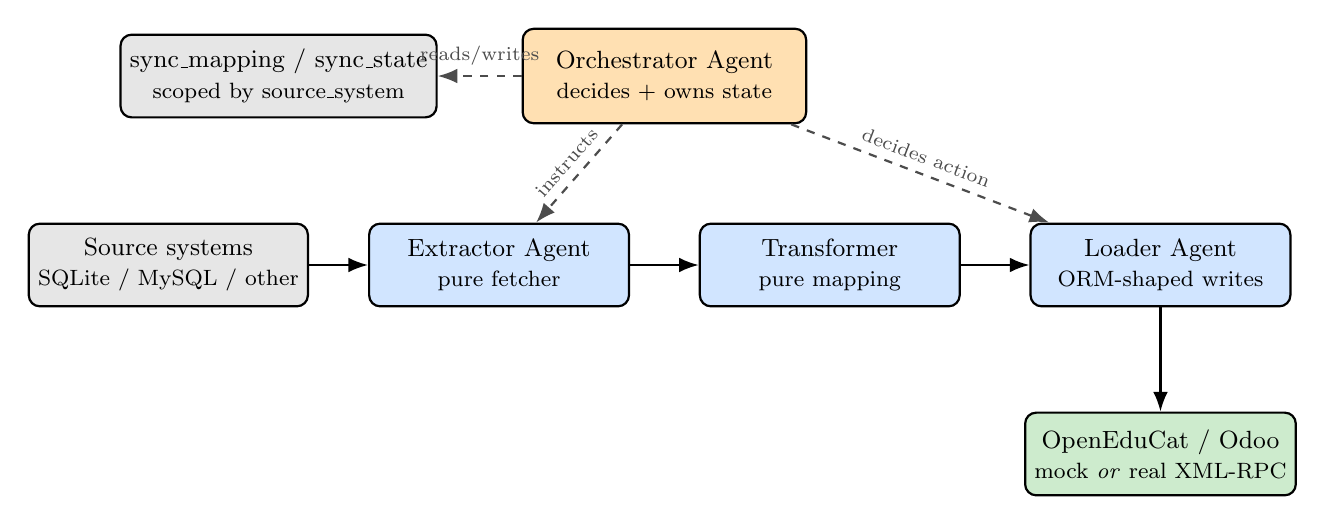
\begin{tikzpicture}[node distance=1.5cm]
\node[comp] (src) at (0,0) {Source systems\\\footnotesize SQLite / MySQL / other};
\node[agentbox] (ext) at (4.2,0) {Extractor Agent\\\footnotesize pure fetcher};
\node[agentbox] (tr) at (8.4,0) {Transformer\\\footnotesize pure mapping};
\node[agentbox] (ld) at (12.6,0) {Loader Agent\\\footnotesize ORM-shaped writes};
\node[realbox] (tgt) at (12.6,-2.4) {OpenEduCat / Odoo\\\footnotesize mock \emph{or} real XML-RPC};
\node[orchbox] (orch) at (6.3,2.4) {Orchestrator Agent\\\footnotesize decides + owns state};
\node[comp] (store) at (1.4,2.4) {sync\_mapping / sync\_state\\\footnotesize scoped by source\_system};

\draw[solidarr] (src) -- (ext);
\draw[solidarr] (ext) -- (tr);
\draw[solidarr] (tr) -- (ld);
\draw[solidarr] (ld) -- (tgt);
\draw[dashedarr] (orch) -- node[above,font=\scriptsize,sloped]{instructs} (ext);
\draw[dashedarr] (orch) -- node[above,font=\scriptsize,sloped]{decides action} (ld);
\draw[dashedarr] (orch) -- node[above,font=\scriptsize]{reads/writes} (store);
\end{tikzpicture}
\caption{The pipeline in Revision~2. The agents are unchanged from Revision~1; what became
pluggable is what sits at each end -- any adapter satisfying the \texttt{SourceAdapter} contract
on the left, either the mock or a real Odoo instance on the right.}
\end{figure}

\subsection{Three independently-owned local stores}

The separation of concerns is enforced at the storage layer:

\begin{itemize}[leftmargin=1.4em]
    \item \ttu{data/pieas.db} -- the dummy PIEAS source (used when \ttu{--source pieas}). Only
          \texttt{ExtractorAgent} opens it, and only through the selected adapter module.
    \item \ttu{data/openeducat_mock.db} -- the mock target (used when \ttu{--target mock}). Only
          the Loader and the read-only Validator touch it.
    \item \ttu{data/orchestrator_state.db} -- \ttu{sync_mapping} and \ttu{sync_state}. Only the
          Orchestrator imports \ttu{sync_store.py} at all.
\end{itemize}

No other agent module has a code path to open the ``wrong'' store. When running against real
infrastructure, the first two are replaced by a real MySQL server and a real Odoo instance
respectively; the third remains local, because it is this pipeline's own private bookkeeping,
not anybody's system of record.

% =========================================================================
\section{Agent-by-Agent Breakdown}
% =========================================================================

\begin{table}[H]
\centering
\small
\begin{tabular}{@{}p{2.6cm}p{11.4cm}@{}}
\toprule
\textbf{Agent} & \textbf{Responsibility} \\
\midrule
\textbf{Extractor} & The only agent that touches a source system. Pure fetcher: given an
instruction (\ttu{fetch_changed}, \ttu{fetch_page}, \ttu{fetch_ids}) it returns raw rows and holds
no state between calls. In Revision~2 it takes an injected adapter module, so pointing it at
MySQL instead of SQLite required no change to the agent itself. \\
\textbf{Transformer} & Pure function from a source-shaped dict to a target-shaped dict, per entity
type. Identical input always produces identical output, with no I/O and no awareness of create
vs.\ update. Against the real target the function is \emph{compiled from a reviewed JSON mapping}
rather than hand-written, but it remains a pure function of the same shape. \\
\textbf{Loader} & Writes into the target through an ORM-shaped client, executing exactly the
action it is told: \texttt{create}, \texttt{update} (write), or \texttt{archive}
(write \ttu{active=False}). Makes no decisions about which applies. \\
\textbf{Orchestrator} & The only decision-maker. Owns \ttu{sync_mapping}/\ttu{sync_state}
exclusively, decides what to fetch and when, classifies each record
\texttt{create}/\texttt{update}/\texttt{unchanged}, and (in the deletion cycle)
\texttt{archive}. Each instance is scoped to one \ttu{source_system}. \\
\textbf{Validator} \newline \footnotesize(optional, \S3.4) & Re-reads a record after a Loader write
and confirms it matches what was sent. Observes after the fact; never blocks or retries a write
itself, and its findings are advisory entries in the run report. \\
\bottomrule
\end{tabular}
\caption{The five agents and their strictly non-overlapping responsibilities.}
\end{table}

\subsection{Illustrative excerpt: the Orchestrator's classification logic}

This is the decision the entire system exists to make -- \texttt{create} vs.\ \texttt{update}
vs.\ \texttt{unchanged} for every fetched source row, by looking up the mapping table. Note that
it reads \ttu{record["source_id"]}, not \ttu{record["pieas_id"]}: every adapter aliases its own
primary key to that generic name, which is what leaves this method with no source-specific
assumption in it.

\begin{lstlisting}[caption={\ttu{OrchestratorAgent.classify_records} (abridged).}]
for record in records:
    source_id = record["source_id"]
    business_fields = {k: v for k, v in record.items() if k != "last_updated"}
    h = store.content_hash(business_fields)
    mapping = store.get_mapping(self._conn, self._source_system, source_id, entity_type)
    if mapping is None:
        action, openeducat_id = "create", None
    elif mapping["content_hash"] == h:
        action, openeducat_id = "unchanged", mapping["openeducat_id"]
    else:
        action, openeducat_id = "update", mapping["openeducat_id"]
\end{lstlisting}

% =========================================================================
\section{Multi-Source Generalization}
\label{sec:multisource}
% =========================================================================

\subsection{The formal contract}

Revision~1's ``any source system works'' was an unenforced convention: two adapter modules
happened to expose identical function signatures, but nothing checked that, and nothing told a
new adapter author what was actually required. \ttu{source_adapter.py} now makes the contract
explicit and runtime-checkable:

\begin{lstlisting}[caption={The \texttt{SourceAdapter} Protocol -- the read path the Extractor
actually needs.}]
@runtime_checkable
class SourceAdapter(Protocol):
    def get_connection(self, conn_info: Optional[Any] = None) -> Any: ...
    def fetch_changed(self, conn: Any, table: str, watermark: Optional[datetime]) -> list[dict]: ...
    def fetch_page(self, conn: Any, table: str, limit: int, offset: int) -> list[dict]: ...
    def fetch_ids(self, conn: Any, table: str) -> list[str]: ...
\end{lstlisting}

A companion \ttu{check_adapter()} raises an error naming exactly which function is missing,
rather than letting a new adapter fail confusingly deep inside the Extractor the first time a
particular method happens to be called. Seeding and mutation helpers
(\ttu{insert_*}, \ttu{update_fields}, \ttu{delete_row}) are deliberately \emph{not} part of the
contract: they are test/demo scaffolding, and a real production source adapter should not be
able to write back into the source system at all.

\subsection{The wire format, and eliminating \texttt{pieas\_id}}

The contract is not only about function names. Every adapter must also alias, in its fetch
functions' output, its own primary key to \ttu{source_id} and its own change-tracking column to
\ttu{last_updated}, regardless of what the source calls them natively. That one discipline is
what allows the Orchestrator, the state store, the graph, the Loader, and the Validator to
contain no source-specific field name whatsoever.

Getting there required a codebase-wide rename in Revision~2. Every \ttu{pieas_id} reference was
inventoried and then classified into exactly one of three categories, only the first of which
was renamed:

\begin{table}[H]
\centering
\small
\begin{tabular}{@{}p{3.9cm}p{4.4cm}p{6.2cm}@{}}
\toprule
\textbf{Category} & \textbf{Example} & \textbf{Action} \\
\midrule
Generic pipeline code & Orchestrator, graph, sync store, Loader, Validator &
\textbf{Renamed} to \ttu{source_id} -- these must know nothing about PIEAS \\
Source-specific models & \ttu{PieasStudent.pieas_id} &
\textbf{Left alone} -- a PIEAS model is correctly allowed to name its own PIEAS key \\
Mock target's own schema & the \ttu{op_student.pieas_id} column &
\textbf{Left alone} -- that is the mock's private implementation detail; renaming it is churn with
no generalization benefit \\
\bottomrule
\end{tabular}
\caption{How the rename was scoped. Distinguishing these three cases was the substance of the
work; a blind find-and-replace would have been wrong in two of them.}
\end{table}

\subsection{Logical source systems vs.\ physical backing stores}

A distinction that matters, and which the CLI surfaces directly. \ttu{sync_mapping} and
\ttu{sync_state} are scoped by \ttu{source_system} -- a \emph{logical} identity -- not by the
database technology behind it:

\begin{itemize}[leftmargin=1.4em]
    \item \ttu{pieas_source.py} (SQLite) and \ttu{pieas_source_mysql.py} (MySQL) are two
          \emph{physical} backing stores for \emph{one} logical source system, \ttu{"pieas"}.
          They deliberately share the same mapping rows and the same watermark.
    \item \ttu{example_univ_source.py} is a genuinely different logical source system, and
          therefore gets its own mapping rows and its own watermark for the same entity types.
\end{itemize}

Two tests exist specifically to prove the isolation holds
(\ttu{test_mapping_scoped_by_source_system}, \ttu{test_watermark_scoped_by_source_system}):
before this change, the unique constraint was \ttu{(pieas_id, entity_type)}, so a second
university syncing ``student'' would have fought over the same rows as PIEAS.

\subsection{Why MySQL for the real source}

The real source database is MySQL, and that is a deliberate choice rather than an incidental
one. Odoo's own backing store is PostgreSQL. Had the stand-in source also been PostgreSQL, the
setup would have quietly understated exactly the cross-system heterogeneity this project exists
to prove out -- a real legacy campus system and a modern ERP would almost never share database
technology. Choosing a different engine forced the adapter layer to actually earn its keep:
MySQL returns \texttt{datetime} objects where SQLite returns ISO strings, which the adapter must
normalise; and MySQL's native \ttu{ON UPDATE CURRENT_TIMESTAMP(6)} column attribute replaces the
SQLite build's hand-written trigger.

% =========================================================================
\section{The Real Target: Odoo + OpenEduCat}
\label{sec:realtarget}
% =========================================================================

\ttu{openeducat_client.py} contains two implementations of one method surface
(\texttt{create}, \texttt{write}, \texttt{archive}, \texttt{read}, \ttu{search_read},
\ttu{search_count}):

\begin{itemize}[leftmargin=1.4em]
    \item \textbf{\texttt{OpenEduCatClient}} -- SQLite-backed mock. The entire test suite runs
          against this, which is why the suite needs no live services.
    \item \textbf{\texttt{OdooXmlRpcClient}} -- real XML-RPC against a self-hosted Odoo~19.0 +
          OpenEduCat~19.0 instance: authenticate once against \texttt{common} for a uid, then
          \ttu{execute_kw(db, uid, password, model, method, args, kwargs)} for everything else.
\end{itemize}

\subsection{External-ID tracking via \texttt{ir.model.data}}

Real OpenEduCat models have no field in which to store a foreign system's key. Rather than
adding a custom column to a third-party module's schema, the real client registers each link
through Odoo's own external-ID mechanism, \ttu{ir.model.data}, under a dedicated module name
\ttu{openedu_sync}. This is the standard Odoo-native answer to the problem, and it has the
useful property of being discoverable from the Odoo side without depending on this pipeline's
private \ttu{sync_mapping} store.

That property was tested unintentionally but conclusively. After the \ttu{pieas_id} $\rightarrow$
\ttu{source_id} rename, the local state store's schema no longer matched its existing file, and
the file had to be rebuilt. Because the stored external-ID \emph{value} format
(\ttu{f"{model}_{external_id}"}) had not changed -- only the Python dictionary key had -- every
previously-migrated record was still discoverable. A reconciliation script recovered all
\textbf{89} of them (59~students, 17~faculty, 13~courses) with zero missing.

\subsection{Where the real target's schema diverges from the mock}

Testing against the real instance surfaced a modelling mismatch that the mock had papered over:
\textbf{PIEAS's ``course'' is not Odoo's \ttu{op.course}}. In real OpenEduCat, \ttu{op.course}
represents a degree programme, while an individual taught subject is \ttu{op.subject}. The mock
maps course to \ttu{op.course}; the real target maps it to \ttu{op.subject}, handled by a single
override in the CLI:

\begin{lstlisting}[caption={The one place the two targets' model maps diverge.}]
REAL_MODEL_FOR_ENTITY = {**OPENEDUCAT_MODEL_FOR_ENTITY, "course": "op.subject"}
\end{lstlisting}

The mock's own mapping was deliberately left as-is. Changing it would have meant rewriting the
mock's SQLite schema and a run of tests, to make a test double more faithful to a system it is
explicitly standing in for -- with the real path already covered by the override.

% =========================================================================
\section{The Mapping-Authoring Tool}
\label{sec:mapping}
% =========================================================================

\subsection{What the evidence actually justified}

The internship's original direction included an ``LLM-assisted Transformer for messy or
ambiguous field mapping.'' Running bulk migration against the real instance produced evidence
that complicates that premise. Every real mismatch encountered was a \emph{lookup}, not a
judgement call:

\begin{table}[H]
\centering
\small
\begin{tabular}{@{}p{6.4cm}p{7.6cm}@{}}
\toprule
\textbf{Mismatch found against real OpenEduCat} & \textbf{Nature of the problem} \\
\midrule
\ttu{roll_number} $\rightarrow$ \ttu{gr_no} & Rename, visible directly in \ttu{fields_get}'s label \\
\ttu{gender} codes differ between \ttu{op.student} (\texttt{m}/\texttt{f}/\texttt{o}) and
\ttu{op.faculty} (\texttt{male}/\texttt{female}) \emph{on the same instance} &
Value-domain mismatch, visible directly in \ttu{fields_get}'s selection list \\
\ttu{department} / \ttu{batch_year} have no plain-field equivalent on \ttu{op.student} &
Structural/relational modelling gap -- needs ORM knowledge, not fuzzy matching \\
\bottomrule
\end{tabular}
\caption{None of these required live natural-language reasoning per record. They required schema
introspection plus a static lookup table.}
\end{table}

The conclusion drawn -- and implemented -- is that an LLM belongs at \textbf{design time, not
runtime}. Onboarding a new university still means a human working out ``their \ttu{student_no}
is our \ttu{gr_no}'' across dozens of fields, once. An LLM given both schemas completely and
structurally (via introspection, not guesswork) is well suited to drafting that mapping for a
human to review. It is emphatically not suited to re-deciding it on every record of every sync
run, where determinism, testability, and auditability matter more.

\subsection{How it works}

\ttu{mapping_authoring.py} extracts the source schema from the Pydantic models and the target
schema live from the real instance via \ttu{fields_get}, prompts Gemini for a structured
\texttt{MappingProposal}, and validates the response against that schema. The output is written
to \ttu{mappings/*_gemini_draft.json}. A human reviews it and approves a working copy at
\ttu{mappings/*_pieas.json}, which \ttu{compile_mapping()} turns into the actual pure transform
function used for \ttu{--target real}.

Three properties were treated as non-negotiable:

\begin{enumerate}[leftmargin=1.4em]
    \item \textbf{Never a runtime component.} It is never called during a \ttu{run_cycle}.
    \item \textbf{Never authoritative.} Output is always a draft pending human review. The
          \ttu{*_gemini_draft.json} files are kept in the repository as an honest historical
          record of what the model actually proposed, and are deliberately \emph{not} updated when
          the approved mappings change.
    \item \textbf{Never invents data.} A target-required field with no source equivalent is
          reported under \ttu{unmapped_required_target_fields} with an explanatory note, not
          silently defaulted. Where a default genuinely is applied (e.g.\ \ttu{op.subject}'s
          required \ttu{subject_type}), the mapping file records it as a disclosed assumption.
\end{enumerate}

\subsection{A note on scope discipline}

One finding from this work is worth recording because it cuts against the tool's own premise.
An early ``faculty gender gap'' was treated as an immovable real-world constraint --
PIEAS supposedly had no gender field for faculty, so \ttu{op.faculty.gender} could not be
populated. It was then pointed out, correctly, that the dummy PIEAS schema was authored by this
project itself; the gap was self-inflicted, not a fact about PIEAS. The schema was extended and
the ``gap'' disappeared. The lesson generalises: when working against a stand-in for a real
system, it is easy to mistake an arbitrary property of your own test fixture for a genuine
external constraint.

% =========================================================================
\section{The LangGraph Orchestration Layer}
% =========================================================================

\subsection{Why one graph, not three}

All three cycles share the same Extractor $\rightarrow$ Transformer $\rightarrow$ Loader
pipeline and differ only in what the Orchestrator asks the Extractor to fetch and what it does
with the result. They are therefore one \texttt{StateGraph} whose nodes branch on
\ttu{state["mode"]}, not three separate graphs.

\begin{figure}[H]
\centering
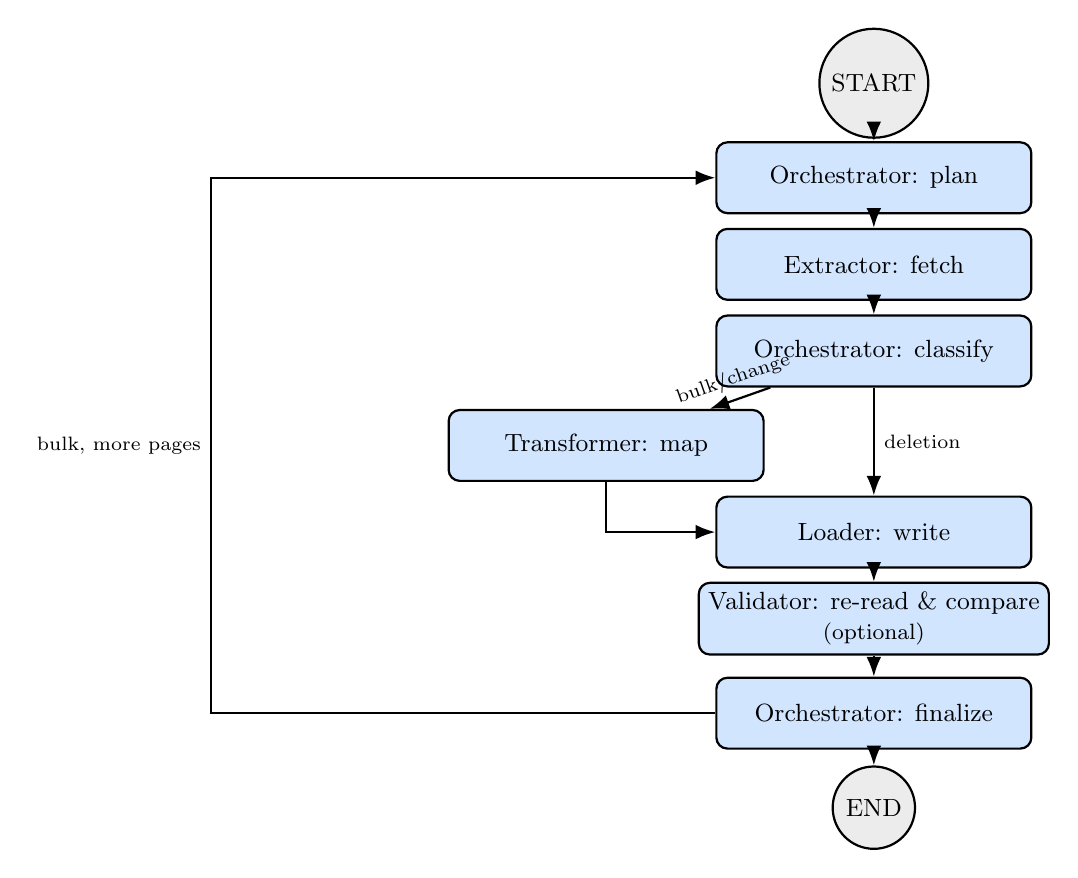
\begin{tikzpicture}[node distance=0.9cm]
\node[term] (start) at (0,6.8) {START};
\node[stage] (plan) at (0,5.6) {Orchestrator: plan};
\node[stage] (extract) at (0,4.5) {Extractor: fetch};
\node[stage] (classify) at (0,3.4) {Orchestrator: classify};
\node[stage] (transform) at (-3.4,2.2) {Transformer: map};
\node[stage] (load) at (0,1.1) {Loader: write};
\node[stage] (validate) at (0,0.0) {Validator: re-read \& compare\\\footnotesize (optional)};
\node[stage] (finalize) at (0,-1.2) {Orchestrator: finalize};
\node[term] (end) at (0,-2.4) {END};

\draw[solidarr] (start) -- (plan);
\draw[solidarr] (plan) -- (extract);
\draw[solidarr] (extract) -- (classify);
\draw[solidarr] (classify) -- node[above,font=\scriptsize,sloped]{bulk/change} (transform);
\draw[solidarr] (transform) |- (load);
\draw[solidarr] (classify) -- node[right,font=\scriptsize]{deletion} (load);
\draw[solidarr] (load) -- (validate);
\draw[solidarr] (validate) -- (finalize);
\draw[solidarr] (finalize) -- (end);
\draw[solidarr] (finalize.west) -- ++(-6.4,0) |- node[left,font=\scriptsize,pos=0.25]{bulk, more pages} (plan.west);
\end{tikzpicture}
\caption{The single pipeline state machine. Passing \texttt{validator=None} removes the validate
node from the graph entirely rather than making it a no-op, so the optional-agent boundary is
structural rather than a runtime flag.}
\end{figure}

\subsection{A subtlety worth documenting: pagination and running totals}

Bulk migration loops \texttt{plan} $\rightarrow$ \dots $\rightarrow$ \texttt{finalize} once per
page, and LangGraph state keys are last-write-wins with no reducer. Per-page results would
therefore be clobbered by the following page. The fix is that \ttu{finalize_node} accumulates
running totals rather than writing per-page values:

\begin{lstlisting}[caption={Running totals in \ttu{finalize_node}, without which paginated bulk
migration would report only the final page.}]
update = {
    "total_fetched":   state.get("total_fetched", 0)   + page_fetched,
    "total_created":   state.get("total_created", 0)   + page_created,
    "total_updated":   state.get("total_updated", 0)   + page_updated,
    "total_unchanged": state.get("total_unchanged", 0) + page_unchanged,
    "total_archived":  state.get("total_archived", 0)  + page_archived,
}
\end{lstlisting}

The same reasoning applies to the watermark, which is carried across pages as a running maximum
rather than overwritten.

% =========================================================================
\section{Change Detection and Deletion Detection}
\label{sec:change-deletion}
% =========================================================================

\subsection{Change detection: timestamp watermark}

Both alternatives the report weighs require a column on the source side. A boolean dirty flag
has a reset race condition: between reading the flagged rows and clearing the flags, a further
edit can land and be silently lost. A timestamp watermark has no such window, so that is what
is implemented -- one \ttu{last_updated} per row, one \ttu{last_synced_at} watermark per
\ttu{(source_system, entity_type)}.

\begin{lstlisting}[language=SQL, caption={The change query, in essence.}]
SELECT * FROM students
WHERE last_updated > :watermark
ORDER BY last_updated ASC;
\end{lstlisting}

The watermark then advances to the \textbf{maximum \ttu{last_updated} actually processed in the
run}, not to wall-clock \texttt{NOW()} -- safer against a row changing again mid-run.

\subsection{Deletion detection: full ID list, compared locally}

A filtered \ttu{last_updated} query can never see a deletion: a row that no longer exists cannot
match a \texttt{WHERE} clause. This is a structural property, not a tuning problem, and it is
why deletion needs its own cycle. That cycle fetches the \emph{full} current ID list from the
source and computes a set difference against \ttu{sync_mapping} locally -- equivalent to the
report's \texttt{LEFT JOIN \dots\ WHERE \dots\ IS NULL}, but without requiring a live
cross-database join between two systems that cannot see each other.

One test exists purely to assert this property: it proves the change cycle \emph{cannot} detect
a deletion, so that the separate cycle can never be mistaken for redundancy by a future reader.

\subsection{What happens to a detected deletion}

Archive (\ttu{active=False}), never hard-delete. This preserves history and is reversible if the
``deletion'' turns out to have been a rename or a data-entry correction. It is also exactly what
Odoo's own \ttu{active} field is designed for, so the behaviour is identical against the mock and
the real instance.

% =========================================================================
\section{Reference Data and Cross-Entity Dependencies}
\label{sec:refdata}
% =========================================================================

\subsection{Marks: the report's own example, and the first relational entity}

The source report's problem statement uses \emph{``a quiz mark is updated''} as its worked
example of an ongoing change, yet Revision~1 synced only students, faculty, and courses.
Revision~2 adds \texttt{mark} as a fourth entity type -- and doing so exposed a structural
assumption the pipeline had not previously had to confront.

The first three entities are flat and mutually independent: a faculty row can be synced whether
or not any student has been. A mark cannot. It is meaningless without the student who sat the
exam and the subject it was sat in, both of which must already exist on the target. That makes
\ttu{ENTITY_TYPES} an \textbf{ordered} tuple rather than an incidental one, with \texttt{mark}
last, which is what lets \ttu{--entity all} complete in a single pass.

The source tables declare real foreign keys with \ttu{ON DELETE CASCADE}, so deleting a student
genuinely removes their marks -- and the deletion cycle then archives those marks on the target,
without needing any special knowledge that a cascade happened. It sees only that some IDs it has
mappings for are no longer in the source's ID list, which is exactly what the report's
Section~5.3 design already handles.

\subsection{Shared reference records}

Some source values do not name a field on the target at all -- they name a \emph{shared record}
that many source rows point at. \ttu{department} is not a field on real \ttu{op.student}; it is
reached through an \ttu{op.student.course} enrollment $\rightarrow$ \ttu{op.batch}
$\rightarrow$ \ttu{op.course} chain. Revision~1 flagged these as \texttt{unmapped} with an
explanatory note, which was honest but meant a student synced to the real target arrived with no
department, batch, or enrollment at all.

These now use a \texttt{reference} handling, which deliberately mirrors the existing
\texttt{external\_id} sentinel rather than inventing a second mechanism: the compiled transform
passes the value through under a \ttu{__ref__} prefix, and the client resolves it get-or-create
style. The placement follows directly from the report's own agent boundaries:

\begin{table}[H]
\centering
\small
\begin{tabular}{@{}p{3.2cm}p{10.8cm}@{}}
\toprule
\textbf{Candidate layer} & \textbf{Why not / why yes} \\
\midrule
Transformer & \textbf{No.} Resolving a reference means querying the target. The report
(Section~3.3) requires the Transformer to be a pure function; giving it I/O would break the one
property that makes it trivially testable. \\
Loader & \textbf{No.} Its job is to execute exactly the action it was handed. Deciding that a
department must be created first is not that. \\
Client & \textbf{Yes.} The client \emph{is} the target adapter. ``How this particular target
represents a student's department'' is precisely its concern, and it is already the only layer
allowed to talk to the target. \\
\bottomrule
\end{tabular}
\caption{Where reference resolution belongs, argued from the report's existing boundaries rather
than from convenience.}
\end{table}

Two properties fall out of this that are worth stating explicitly. First, resolution is
\textbf{idempotent and shared}: every Physics 2027 student resolves to the same one
\ttu{op.batch}, and re-syncing an unchanged student does not add a second enrollment. Second,
cross-entity references need \textbf{no second mapping store} -- a mark's student and subject are
resolved through the very same \ttu{ir.model.data} external IDs the pipeline registered when it
synced them, which is the same mechanism that survived the \ttu{source_id} rename intact.

A mark whose student has not been synced yet fails with an error naming the problem, rather than
writing a dangling foreign key or silently defaulting. That is the same stance taken everywhere
else in this project: fail loudly rather than corrupt quietly.

\subsection{Constants for required target fields}

\ttu{op.exam.attendees} requires a \ttu{status} (present/absent) that PIEAS has no equivalent
for -- it records the mark, not attendance. Approved mappings may therefore carry a
\ttu{constant_fields} block, and \ttu{status} is set to \texttt{present} on the reasoning that a
recorded mark implies the student sat the paper.

This is deliberately \emph{not} part of \texttt{MappingProposal}, the LLM's output schema. The
tool's job is to \textbf{report} a required target field it has no source for, under
\ttu{unmapped_required_target_fields}; deciding what constant belongs there is a human review
decision. Keeping it out of the proposal schema is a structural way of enforcing the project's
standing rule that the model never fabricates data -- it can raise the question, but it cannot
answer it.

% =========================================================================
\section{Reconciliation and Cutover Verification}
\label{sec:reconcile}
% =========================================================================

Migration has a phase the first report did not address: the moment of \textbf{cutover}, when
OpenEduCat becomes the system of record. Before that, somebody must be able to answer ``is
everything actually across?'' with evidence rather than optimism.

The \texttt{reconcile} command is that evidence. It is strictly read-only -- it writes nothing,
to any system -- and compares the source's live ID list, \ttu{sync_mapping}, and the target's
actual state, reporting four categories of drift:

\begin{table}[H]
\centering
\small
\begin{tabular}{@{}p{3.4cm}p{10.6cm}@{}}
\toprule
\textbf{Category} & \textbf{Meaning} \\
\midrule
\ttu{not_synced} & Present at the source but absent from \ttu{sync_mapping} -- a bulk or change
cycle should have created this and did not. \\
\ttu{missing_target} & \ttu{sync_mapping} points at a target record that no longer exists --
e.g.\ deleted directly in OpenEduCat, outside this pipeline. \\
\ttu{stale_archived} & Still present at the source but archived on the target. \\
\ttu{should_be_archived} & Gone from the source but still active on the target -- the deletion
cycle that should have handled it has not run, or did not get that far. \\
\bottomrule
\end{tabular}
\caption{The drift taxonomy. \texttt{reconcile} exits with status~1 if any category is non-empty,
so it can gate a cutover in a deployment script or CI job.}
\end{table}

It is deliberately a \emph{verify} tool, not a \emph{fix} tool: re-running \texttt{sync} or
\texttt{deletion-check} is what closes any drift it reports. Keeping detection and remediation
separate means the audit can be trusted to be non-destructive and run freely at any time.

\subsection{First real run, and an honest caveat}

Run against the real Odoo instance, \texttt{reconcile} reported \texttt{faculty} and
\texttt{course} clean and flagged exactly one student, \ttu{PIEAS-STU-MYSQL-NEW-001}, as
\ttu{should_be_archived}. Investigation confirmed the finding was correct and the cause benign:
that record exists only in the MySQL backing store, not the SQLite one, and the two share a
single logical \ttu{source_system} by design. Reconciling one physical backend against mappings
partly written by the other necessarily reports the difference.

A second caveat is documented in the command's own help text: \ttu{sync_mapping} scopes by
\ttu{source_system}, \emph{not} by target, because the design assumes one live target per
deployment. Running \texttt{reconcile} with a different \texttt{--target} than the one that wrote
the current mapping rows compares stored IDs against the wrong system's ID space and reports
every row as \ttu{missing_target}. That is a mismatched invocation, not drift, and saying so
plainly in the tool is better than letting a future operator lose an afternoon to it.

% =========================================================================
\section{Production Hardening}
\label{sec:hardening}
% =========================================================================

\subsection{Retry and backoff}

Every RPC the real client makes now funnels through an exponential-backoff wrapper. The
important design decision is what is \emph{not} retried:

\begin{lstlisting}[caption={Transient failures only. \texttt{xmlrpc.client.Fault} is deliberately
excluded.}]
_TRANSIENT_RPC_EXCEPTIONS = (
    ConnectionError, TimeoutError, OSError, socket.error,
    http.client.HTTPException, xmlrpc.client.ProtocolError,
)
\end{lstlisting}

\texttt{xmlrpc.client.Fault} is Odoo's own application-level rejection -- a failed validation, a
uniqueness violation. Retrying it would repeat the same rejection three times, turning one clear
error into three and recovering from nothing. The wrapper covers reads as well as writes, since a
dropped connection can just as easily hit the Validator's read-back as a Loader write.

\subsection{Structured logging}

The existing Rich console output serves a human watching a terminal. It does not serve an
operator who is not watching one. \ttu{logging_config.py} adds a stdlib-only JSON formatter
emitting one object per event, suitable for shipping to an aggregator:

\begin{lstlisting}[style=termstyle,caption={A real \ttu{cycle_completed} event.}]
{"timestamp": "2026-08-10T09:45:30.490108+00:00", "level": "INFO",
 "logger": "openedu_orchestrator.graph", "message": "cycle_completed",
 "mode": "change", "entity_type": "faculty", "duration_seconds": 0.010438,
 "n_fetched": 1, "n_created": 0, "n_updated": 0, "n_unchanged": 1,
 "n_archived": 0, "pages": 1, "error_count": 0, "validation_issue_count": 0}
\end{lstlisting}

Instrumented events are \ttu{cycle_started} and \ttu{cycle_completed} in \ttu{run_cycle},
\ttu{rpc_retry} and \ttu{rpc_retry_exhausted} in the retry wrapper, and \ttu{load_write_failed}
on Loader write exceptions. Verbosity is controlled by \ttu{OPENEDU_LOG_LEVEL}.

\subsection{Credentials out of source control}

Odoo and MySQL credentials now load from \ttu{OPENEDU_ODOO_*} and \ttu{OPENEDU_PIEAS_MYSQL_*}
environment variables, with the existing local-development values retained as fallbacks so the
default workflow is unchanged. A committed \ttu{.env.example} documents every variable;
\ttu{.env} itself is git-ignored. The override path was verified rather than assumed: setting
\ttu{OPENEDU_ODOO_USERNAME} to a nonexistent user produces an authentication failure naming that
user, confirming the value is genuinely reaching the client.

This is deliberately the \emph{generic} mechanism only. Integration with a specific secrets
manager (AWS Secrets Manager, HashiCorp Vault, etc.) is left open, because that choice depends on
a deployment target that has not yet been decided -- see Section~\ref{sec:remaining}.

\subsection{Continuous integration}

\ttu{.github/workflows/ci.yml} runs the full suite on Python~3.11 and~3.12 for every push and
pull request to \texttt{master}. This is only possible because the suite is entirely
self-contained: every test runs against SQLite fixtures in a \ttu{tmp_path}, with no live Odoo or
MySQL dependency. Before committing the workflow, the exact install-and-test sequence was
rehearsed in a throwaway clean virtual environment to confirm \ttu{requirements.txt} alone is
sufficient.

% =========================================================================
\section{Bugs Found Only By Testing Against Real Infrastructure}
\label{sec:realbugs}
% =========================================================================

This section is the empirical justification for the whole real-infrastructure exercise. Each of
the following was invisible to the mock and to the test suite, and each was found by actually
running the pipeline against a live system.

\begin{table}[H]
\centering
\small
\begin{tabular}{@{}p{4.5cm}p{9.5cm}@{}}
\toprule
\textbf{Defect} & \textbf{Detail and resolution} \\
\midrule
\ttu{write()} did not strip the external-ID sentinel &
\texttt{create()} had special-case handling to pop the sentinel key before writing;
\texttt{write()} did not. Every real \emph{update} therefore failed with ``Invalid field''.
The mock silently tolerated the extra key. Fixed by mirroring the logic in \texttt{write()}. \\
\midrule
\ttu{fields_get} argument unpacking &
Passing a list of field names as \texttt{args} caused Odoo to unpack them as separate positional
arguments rather than one list argument. Fixed by wrapping in an extra list. A pure
real-API-semantics bug with no mock equivalent. \\
\midrule
\ttu{search_read} crashing on a broken computed field &
Calling \ttu{search_read} without an explicit \texttt{fields} list makes Odoo compute
\emph{every} field, including one in \ttu{openeducat_fees} that raises ``Expected singleton'' on
a multi-record recordset. Surfaced through the new \texttt{status} command. Fixed by adding
\ttu{search_count()} to both clients and using Odoo's native \ttu{search_count} RPC, which never
computes field values -- counting should not require computing fields in the first place. \\
\midrule
Validator false positive on the \ttu{source_id} sentinel &
\ttu{validate_write()} compared every key it sent against the record it read back, including
\ttu{source_id} -- which is popped before writing and registered via \ttu{ir.model.data}, so it is
never a persisted field and can never match. Every real write reported a spurious validation
issue. Fixed by excluding the sentinel from the comparison. This had likely been latent since the
real-target work began, hidden because ad-hoc scripts did not always inspect the
\ttu{validation_issues} count. \\
\midrule
\ttu{LogRecord.created} collision &
The first structured-logging implementation passed a \texttt{created} count via
\ttu{extra={...}}, colliding with \texttt{logging}'s own reserved record-creation-time attribute
and raising \texttt{KeyError} at runtime. Found by running a real sync, not by reading the code.
Fixed by prefixing the count fields (\ttu{n_created}, \ttu{n_updated}, \dots) to avoid the entire
class of collision rather than only this instance. \\
\bottomrule
\end{tabular}
\caption{Five defects that a mock target could not have exposed.}
\end{table}

\subsection{One non-bug, recorded for honesty}

A sixth failure looked like a defect and was not. After the Validator fix, a re-test produced
\texttt{errors=1: ``Registration Number must be unique per student!''}. The cause was a
self-inflicted test-data collision: the MySQL store had been seeded with the same deterministic
Faker seed as the SQLite one, so it contained a record with the same registration number as a
student that had been deleted from SQLite earlier in the session and archived in Odoo. Because
the earlier reconciliation had only recovered records still present in SQLite at that time, that
ID had no local mapping, was classified as a \texttt{create}, and collided with the archived
record. The correct diagnosis was ``an artefact of reusing identical seed data across two demo
backends against a shared target with history'', and it was confirmed by re-running the identical
scenario on a collision-free record, which passed with \texttt{errors=0}. It is recorded here
because distinguishing a real defect from a test-environment artefact is itself part of the work.

% =========================================================================
\section{Design Decisions Carried Over From the Report}
% =========================================================================

\begin{table}[H]
\centering
\small
\begin{tabular}{@{}p{4.6cm}p{9.4cm}@{}}
\toprule
\textbf{Decision point} & \textbf{Resolution (as implemented)} \\
\midrule
Change detection mechanism & Timestamp watermark, not a boolean dirty flag -- avoids the
reset race condition. \\
Deletion detection mechanism & Separate, less-frequent cycle: full ID fetch, compared locally
against \ttu{sync_mapping}. \\
What to do with a detected deletion & Archive (\ttu{active=False}), not hard-delete --
reversible, preserves history. \\
How to write into the target & Through an ORM-shaped interface, never raw SQL. Validated in
Revision~2 against the real instance, where Odoo's ORM genuinely does enforce the constraints
and computed fields this decision was made to preserve. \\
Was a separate Monitor Agent needed? & No -- absorbed by the Orchestrator, which already owns the
state needed for the comparison. \\
\bottomrule
\end{tabular}
\caption{Every major design fork in the source report, and how this implementation resolves it.
Revision~2 changed none of these conclusions; it supplied evidence for them.}
\end{table}

% =========================================================================
\section{Refinements Beyond the Report's Literal Text}
\label{sec:refinements}
% =========================================================================

\begin{enumerate}[leftmargin=1.4em]
    \item \textbf{Watermark advances by processed maximum, not \texttt{NOW()}.} Safer against a
          row changing again mid-run than the report's literal Listing~7.
    \item \textbf{A content-hash check layered on top of the watermark.} A record whose
          \ttu{last_updated} was touched but whose business fields are byte-for-byte identical
          classifies as \texttt{unchanged} rather than \texttt{update}. This also lets bulk
          migration seed the watermark itself, so the first change cycle afterwards need not
          re-fetch and re-classify every just-migrated row merely to discover where to start.
    \item \textbf{Source-system scoping} (Revision~2). The report assumes a single source. Scoping
          state by \ttu{source_system} generalises it to many at the cost of one extra column.
    \item \textbf{A read-only reconciliation command} (Revision~2). The report describes migration
          and steady-state sync but not the verification step between them.
\end{enumerate}

% =========================================================================
\section{Technology Stack}
% =========================================================================

\begin{table}[H]
\centering
\small
\begin{tabular}{@{}p{2.4cm}p{3.2cm}p{7.4cm}@{}}
\toprule
\textbf{Library} & \textbf{Role} & \textbf{Why} \\
\midrule
\texttt{langgraph} & Orchestration state machine & Purpose-built for stateful, branching agent
pipelines; not restricted to LLM-driven agents. \\
\texttt{pydantic} & Typed data models & Malformed records fail loudly at a model boundary rather
than silently corrupting a write. \\
\texttt{sqlite3} (stdlib) & Mock stores & Zero external services needed to run or test. \\
\texttt{pymysql} & Real MySQL source & Deliberately different engine from the target's
PostgreSQL. \\
\ttu{xmlrpc.client} (stdlib) & Real Odoo target & Odoo's own external API protocol. \\
\ttu{google-genai} & Mapping-authoring tool & Design-time only; never in the sync path. \\
\texttt{Faker} & Deterministic dummy data & Reproducible fake records from a fixed seed. \\
\texttt{click} & CLI & Clean subcommands and shared \texttt{--source}/\texttt{--target} options. \\
\texttt{rich} & Console output & Readable tables for \texttt{status} and \texttt{demo}. \\
\texttt{logging} (stdlib) & Structured JSON logs & No new dependency for aggregator-ready output. \\
\texttt{pytest} & Test suite & 104 tests with isolated per-test databases via \ttu{tmp_path}. \\
\bottomrule
\end{tabular}
\caption{Full dependency list (\ttu{requirements.txt}).}
\end{table}

\textbf{Note on ``agentic'':} the sync pipeline itself makes no LLM calls. It is agentic in the
report's own sense -- autonomous, cooperating components with clearly separated responsibilities
and a decision-making Orchestrator -- implemented deterministically so every run is reproducible
and testable. The one LLM component added in Revision~2, the mapping-authoring tool, sits
strictly outside that loop by design and by argued justification (Section~\ref{sec:mapping}).
These are two distinct and legitimate senses of the word, and conflating them would misrepresent
the system in either direction.

% =========================================================================
\section{Testing and Quality Assurance}
\label{sec:testing}
% =========================================================================

\subsection{Suite structure}

\begin{figure}[H]
\centering
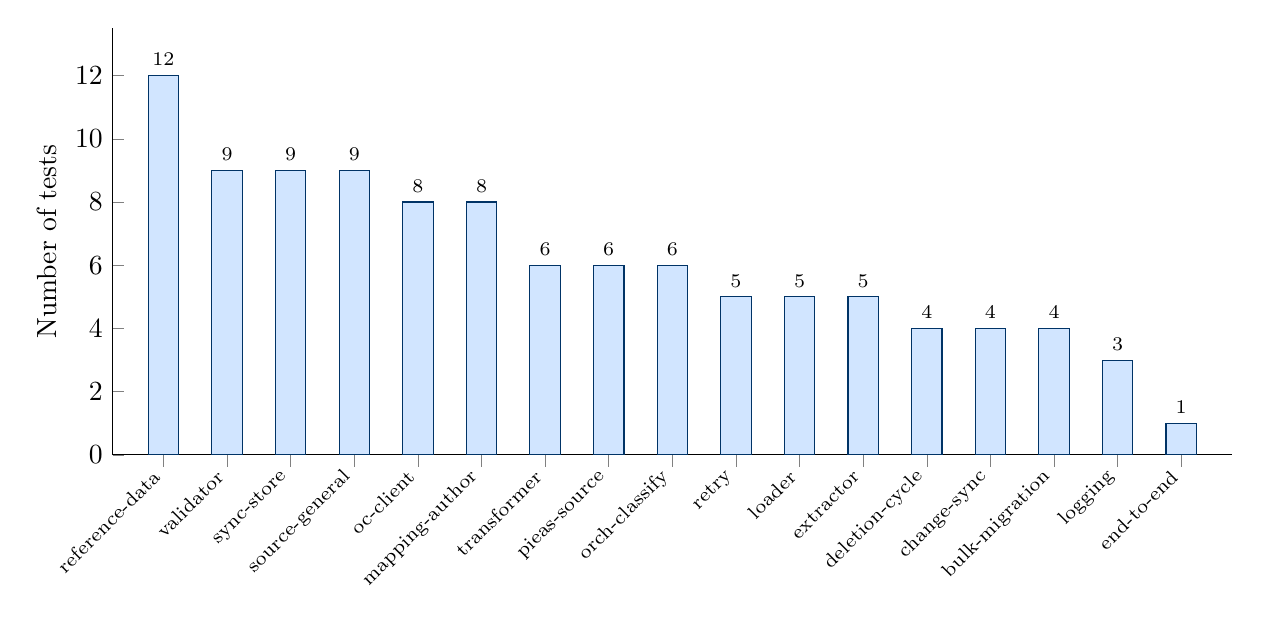
\begin{tikzpicture}
\begin{axis}[
    ybar,
    bar width=11pt,
    width=15.8cm, height=7cm,
    symbolic x coords={reference-data,validator,sync-store,source-general,oc-client,
                        mapping-author,transformer,pieas-source,orch-classify,retry,loader,
                        extractor,deletion-cycle,change-sync,bulk-migration,logging,end-to-end},
    xtick=data,
    x tick label style={rotate=45, anchor=east, font=\scriptsize},
    ylabel={Number of tests},
    ymin=0, ymax=13.5,
    nodes near coords,
    every node near coord/.append style={font=\scriptsize},
    enlarge x limits=0.05,
    axis lines*=left,
    ]
\addplot[fill=AgentBlue, draw=NavyBlue] coordinates {
    (reference-data,12) (validator,9) (sync-store,9) (source-general,9) (oc-client,8)
    (mapping-author,8) (transformer,6) (pieas-source,6) (orch-classify,6) (retry,5) (loader,5)
    (extractor,5) (deletion-cycle,4) (change-sync,4) (bulk-migration,4) (logging,3) (end-to-end,1)
};
\end{axis}
\end{tikzpicture}
\caption{Distribution of the 104-test suite across 17 test modules. Five modules
(\texttt{reference-data}, \texttt{source-general}, \texttt{mapping-author}, \texttt{retry},
\texttt{logging}) are entirely new in Revision~2.}
\label{fig:testchart}
\end{figure}

\begin{table}[H]
\centering
\small
\begin{tabular}{@{}p{6.4cm}p{7.5cm}@{}}
\toprule
\textbf{Test file} & \textbf{What it verifies} \\
\midrule
\ttu{test_pieas_source.py} & Schema, seeding, pagination, watermark filtering, trigger-based
timestamp bump, real row deletion. \\
\ttu{test_openeducat_client.py} & \texttt{create}/\texttt{write}/\texttt{archive}, domain
filtering, unknown-model error handling. \\
\ttu{test_sync_store.py} & Upsert semantics, per-entity scoping, watermark read/write,
content-hash stability, \textbf{and per-\ttu{source_system} isolation of both mappings and
watermarks}. \\
\ttu{test_source_generalization.py} & That the adapter contract is satisfied by each adapter, that
\ttu{check_adapter} rejects an incomplete one, and that two source systems do not interfere. \\
\ttu{test_mapping_authoring.py} & Schema extraction, proposal validation, and that
\ttu{compile_mapping} produces a correct pure transform. \\
\ttu{test_retry.py} & Success without retry, retry-then-succeed, exhaustion, and that
\texttt{Fault} and unrelated exceptions are \emph{not} retried. \\
\ttu{test_logging_config.py} & Valid JSON output, \texttt{extra} fields folded into the payload,
exception rendering. \\
\ttu{test_extractor.py} & Instruction dispatch, statelessness across calls. \\
\ttu{test_transformer.py} & Per-entity field mapping, purity, unknown-entity error. \\
\ttu{test_loader.py} & Create/update/archive execution, graceful failure on a bad update. \\
\ttu{test_orchestrator_classification.py} & create/update/unchanged classification,
deletion-candidate detection, per-entity scoping, bulk-mode flip. \\
\ttu{test_validator.py} & Field-match and mismatch detection, archive-state verification. \\
\ttu{test_graph_bulk_migration.py} & Multi-page pagination totals, per-entity isolation, re-run
idempotency. \\
\ttu{test_graph_change_sync.py} & Edit and new-admission detection, no-op reruns, watermark
monotonicity, cross-entity isolation. \\
\ttu{test_graph_deletion_cycle.py} & Archival correctness, and the structural proof that the
change cycle \emph{cannot} see a deletion. \\
\ttu{test_end_to_end.py} & Full lifecycle across all three entity types in one scenario. \\
\bottomrule
\end{tabular}
\caption{Test file responsibilities.}
\end{table}

\subsection{Verification against real infrastructure}

The automated suite does not touch live systems, so real-target behaviour was verified by
executing the CLI against the running Odoo and MySQL instances and confirming the results by
independent read-back over RPC rather than trusting the pipeline's own report. Representative
results:

\begin{table}[H]
\centering
\small
\begin{tabular}{@{}p{4.0cm}p{4.6cm}p{5.4cm}@{}}
\toprule
\textbf{Scenario} & \textbf{Command} & \textbf{Result} \\
\midrule
Student change cycle, MySQL source, real target &
\ttu{sync --source pieas-mysql --target real --entity student --once} &
\ttu{fetched=1 updated=1 errors=0 validation_issues=0} \\
Course change cycle, real \ttu{op.subject} &
\ttu{sync --target real --entity course --once} &
\ttu{fetched=1 updated=1 errors=0}; new name confirmed on record id~166 by RPC read-back \\
Course deletion cycle, real target &
\ttu{deletion-check --target real --entity course} &
\ttu{fetched=12 archived=1 errors=0}; \ttu{PIEAS-CRS-00008} confirmed \ttu{active=False} on
record id~160 \\
Post-rename reconciliation & ad-hoc, via \ttu{find_by_external_id} &
89 of 89 records recovered (59 student, 17 faculty, 13 course), zero missing \\
\bottomrule
\end{tabular}
\caption{Live verification against the real instance. Each was confirmed by reading the target
back independently, not by trusting the run report.}
\end{table}

One methodological note: verifying an archived record required passing
\ttu{context={"active_test": False}}, because Odoo excludes inactive records from searches by
default. A read-back that returned nothing initially looked like a failed archive and was in fact
a correct archive plus a default search filter -- a distinction worth checking before concluding
anything about archival behaviour.

\subsection{Test run output}

\begin{lstlisting}[style=termstyle,caption={Actual output of the full suite.}]
$ python -m pytest -q
........................................................................ [ 69%]
................................                                         [100%]
104 passed in 4.19s
\end{lstlisting}

% =========================================================================
\section{Command-Line Interface}
% =========================================================================

Two options are shared by the commands that talk to a source or a target, and they are
deliberately orthogonal axes: \texttt{--source} selects which physical store backs the source
system, \texttt{--target} selects the mock or the real Odoo instance. Both were hardcoded before
Revision~2.

\begin{table}[H]
\centering
\small
\begin{tabular}{@{}p{5.2cm}p{8.8cm}@{}}
\toprule
\textbf{Command} & \textbf{Purpose} \\
\midrule
\ttu{seed} & (Re)create the dummy source database with fake data; optionally wipes the mock target
and state store too. \\
\ttu{migrate --entity all} & Run the one-time bulk migration cycle (skips an entity already past
bulk mode). \\
\ttu{mutate --entity student --update N --insert N --delete N} & Simulate the source ``still being
used'': edits, new admissions, removals. \\
\ttu{sync --entity all [--loop --interval S]} & Run the change-detection cycle once, or on a
schedule. \\
\ttu{deletion-check --entity all} & Run the deletion-detection cycle. \\
\ttu{reconcile --entity all} & \textbf{New.} Read-only drift audit; exits 1 if any drift is found. \\
\ttu{status} & Row counts, active/archived counts, mapping counts, and watermarks. \\
\ttu{demo} & One command walking the entire lifecycle end to end. \\
\midrule
\ttu{--source {pieas,pieas-mysql}} & \textbf{New.} Which physical store backs the source system. \\
\ttu{--target {mock,real}} & \textbf{New.} Mock test double, or the live Odoo instance. \\
\bottomrule
\end{tabular}
\caption{\ttu{python -m openedu_orchestrator} command reference.}
\end{table}

\begin{lstlisting}[style=termstyle,caption={Real \texttt{status} output against MySQL source and
real Odoo target. The note is printed by the command itself.}]
$ python -m openedu_orchestrator status --source pieas-mysql --target real
Note: OpenEduCat active/archived counts include any pre-existing target data
(e.g. OpenEduCat's own demo records) -- 'sync_mapping rows' is the accurate
count of what this pipeline itself has actually synced.

Entity   | PIEAS rows | OC active | OC archived | sync_mapping | watermark
---------+------------+-----------+-------------+--------------+----------
student  |         61 |        85 |           2 |           60 | set
faculty  |         18 |        32 |           2 |           17 | set
course   |         14 |       165 |           1 |           13 | set
\end{lstlisting}

That disclaimer matters: against a real instance the raw active/archived counts include
OpenEduCat's own demo data, so they are not a measure of this pipeline's work. Printing the
caveat next to the number is preferable to printing a number that invites a wrong conclusion.

% =========================================================================
\section{Known Characteristics and Limitations}
% =========================================================================

\begin{itemize}[leftmargin=1.4em]
    \item \textbf{Re-archiving a permanently-deleted record.} \ttu{sync_mapping} retains the row,
          so each deletion cycle re-issues a harmless archive write. The cycle's
          \texttt{archived} count therefore reflects ``archive calls issued'', not ``newly
          discovered deletions''. The report's schema defines no way to mark a mapping as already
          handled, and inventing one was avoided.
    \item \textbf{State is scoped by source, not by target.} One live target per deployment is
          assumed. Switching \texttt{--target} without re-syncing produces spurious
          \ttu{missing_target} drift, as documented in Section~\ref{sec:reconcile}.
    \item \textbf{Two backends share one logical source.} \ttu{pieas} and \ttu{pieas-mysql}
          intentionally share \ttu{source_system}, so a record synced from only one of them
          reconciles as drift against the other. This is a consequence of a deliberate design
          choice, not a defect.
    \item \textbf{Mock domain filtering is minimal.} The mock's \ttu{search_read} supports only a
          flat AND of equality conditions -- sufficient here, and irrelevant to the real client,
          which uses Odoo's full domain language.
    \item \textbf{Dummy data, not production data.} Volumes, names, and identifiers are synthetic,
          though department names are drawn from PIEAS's real academic departments for realism.
    \item \textbf{The mapping-authoring tool needs review to be safe.} It is explicitly
          non-authoritative. Its value depends on a human actually reading the draft, and nothing
          in the code can enforce that.
\end{itemize}

% =========================================================================
\section{Remaining Work and Open Decisions}
\label{sec:remaining}
% =========================================================================

\subsection{Deliberate deviations from the report}

Two places where this implementation knowingly differs from the report's literal text. Both are
recorded here rather than left for a reader to discover as apparent oversights.

\begin{table}[H]
\centering
\small
\begin{tabular}{@{}p{3.6cm}p{10.4cm}@{}}
\toprule
\textbf{Report says} & \textbf{What was built, and why} \\
\midrule
The Orchestrator ``owns retry and error-logging logic'' (Section~3.3) &
Error logging is the Orchestrator's, via the run report. \textbf{Retry is not} -- it lives in the
XML-RPC client. A dropped TCP connection is a property of the transport, not a decision about
data, and the Orchestrator is defined as the agent that makes decisions about data. Putting
retry in the client also means it protects the Validator's read-backs, which never pass through
the Orchestrator at all. The distinction the client draws -- retry transient network failures,
never Odoo's own application-level rejections -- is only expressible at that layer. \\
Deletion cycle runs ``once daily'', change cycle ``every 15--60 min'' (Section~4) &
The intervals exist as configuration, but \textbf{no scheduler is implemented}. \ttu{sync --loop}
is a \ttu{time.sleep} loop suitable for a demo, and \texttt{deletion-check} has no loop at all.
Real scheduling belongs to whatever runs the process -- cron, a systemd timer, Celery beat, a
Kubernetes CronJob -- and picking one is part of the deployment decision below. \\
\bottomrule
\end{tabular}
\caption{Knowing deviations, with their justification.}
\end{table}

\subsection{Not implemented}

\begin{itemize}[leftmargin=1.4em]
    \item \textbf{Deployment target.} Kubernetes, a long-running VM with a scheduler, or
          serverless functions on a timer are all viable, and the choice materially affects how
          scheduling, log shipping, and secret injection should be wired. The pipeline is
          agnostic today; committing to one prematurely would embed an unowned assumption.
          \emph{This is the blocker for real scheduling, above.}
    \item \textbf{Secrets-manager integration.} Environment-variable loading is implemented as the
          generic mechanism. Binding to AWS Secrets Manager, HashiCorp Vault, or another specific
          provider follows the deployment decision above.
    \item \textbf{The REST transport.} Section~7 treats OpenEduCat's REST API as a
          ``fallback/alternative transport for the Loader Agent'', while recommending XML-RPC as
          primary. XML-RPC is built and proven; REST is not. The report itself says its
          availability should be confirmed on the actual instance first, which has not been done.
    \item \textbf{``Flag for manual review'' deletions.} Section~5.4 lists this as option~3, ``a
          safer alternative worth mentioning even though archiving was adopted as the default''.
          Archiving is implemented as specified; the manual-review path is not. Given archiving
          is already reversible, this is the lowest-value of the outstanding items.
\end{itemize}

Beyond those, the natural next step is the internship's stated direction: an LLM-driven agentic
layer on top of this deterministic foundation. The foundation was built to make that additive
rather than disruptive -- the mapping-authoring tool is the first instance of the pattern, sitting
outside the sync loop where its non-determinism cannot compromise a data migration.

% =========================================================================
\section{Conclusion}
% =========================================================================

The source report set out to design, not build, an agentic multi-agent system solving two coupled
problems: a one-time bulk migration and an ongoing, agentic synchronization -- including deletion
handling -- between a source system with no API and a target ERP with a well-documented ORM.
Revision~1 of this implementation completed that design into working, tested software against
dummy data and a mock target.

Revision~2's contribution is that the same four agents, unchanged in their responsibilities, now
run against real infrastructure: a real MySQL source, a real Odoo~19.0 + OpenEduCat~19.0 target,
three pluggable source adapters behind a formal contract, reviewed field mappings drafted by an
LLM tool that is kept firmly out of the runtime path, a read-only cutover audit, and the
operational scaffolding -- retries, structured logs, externalised credentials, CI -- that the
difference between a demo and a deployable system actually consists of.

The most useful evidence produced along the way was not any of those features. It was the five
defects in Section~\ref{sec:realbugs}: each one invisible to a passing 57-test suite, each one
found within minutes of pointing the pipeline at a system that had not been built to be
convenient. The agent boundaries the report specified held up under that contact, which is the
strongest thing this report can say about the design it implements.

\appendix
% =========================================================================
\section{Appendix: Project File Tree}
% =========================================================================

\begin{lstlisting}[style=termstyle,basicstyle=\ttfamily\scriptsize\color{white}]
src/openedu_orchestrator/
    config.py                 # paths, entity types, schedules, env-var-backed credentials
    logging_config.py         # structured (JSON) logging setup
    models.py                 # pydantic schemas (PieasStudent/Faculty/Course/Mark, RunReport)
    state.py                  # LangGraph PipelineState TypedDict
    source_adapter.py         # SourceAdapter Protocol -- the multi-source contract
    source_registry.py        # --source name -> adapter module
    pieas_source.py           # dummy SQLite PIEAS adapter
    pieas_source_mysql.py     # real MySQL-backed PIEAS adapter
    example_univ_source.py    # second, distinct logical source system
    openeducat_client.py      # OpenEduCatClient (mock) + OdooXmlRpcClient (real) + retry/backoff
    mapping_authoring.py      # Gemini-assisted mapping proposal + compile_mapping()
    real_target_reference_data.py  # shared reference records + __ref__ resolution dispatch
    sync_store.py             # sync_mapping / sync_state -- Orchestrator-only, source-scoped
    seed.py                   # deterministic Faker-based dummy data generator
    graph.py                  # LangGraph StateGraph wiring + run_cycle()
    cli.py                    # click CLI (seed/migrate/sync/deletion-check/mutate/
                              #            status/reconcile/demo, --source/--target)
    agents/
        extractor.py
        transformer.py
        loader.py
        orchestrator.py
        validator.py
mappings/                     # approved (*_pieas.json) + LLM drafts (*_gemini_draft.json)
.github/workflows/report.yml  # CI: builds this report's PDF
docs/mapping_authoring_tool.md
tests/                        # pytest suite (104 tests, 17 modules)
.github/workflows/ci.yml      # CI: pytest on Python 3.11 + 3.12
.env.example                  # documented environment variables
\end{lstlisting}

\end{document}
